%File: anonymous-submission-latex-2026.tex
\documentclass[letterpaper]{article} % DO NOT CHANGE THIS
\usepackage[submission]{aaai2026}  % DO NOT CHANGE THIS
\usepackage{times}  % DO NOT CHANGE THIS
\usepackage{helvet}  % DO NOT CHANGE THIS
\usepackage{courier}  % DO NOT CHANGE THIS
\usepackage[hyphens]{url}  % DO NOT CHANGE THIS
\usepackage{graphicx} % DO NOT CHANGE THIS
\usepackage{tikz}
\usetikzlibrary{arrows.meta,positioning,fit,shapes}
\urlstyle{rm} % DO NOT CHANGE THIS
\def\UrlFont{\rm}  % DO NOT CHANGE THIS
\usepackage{natbib}  % DO NOT CHANGE THIS AND DO NOT ADD ANY OPTIONS TO IT
\usepackage{caption} % DO NOT CHANGE THIS AND DO NOT ADD ANY OPTIONS TO IT
\frenchspacing  % DO NOT CHANGE THIS
\setlength{\pdfpagewidth}{8.5in} % DO NOT CHANGE THIS
\setlength{\pdfpageheight}{11in} % DO NOT CHANGE THIS
%
% These are recommended to typeset algorithms but not required. See the subsubsection on algorithms. Remove them if you don't have algorithms in your paper.
\usepackage{algorithm}
\usepackage{algorithmic}
\usepackage{algpseudocode}
\usepackage{booktabs}
%
% These are are recommended to typeset listings but not required. See the subsubsection on listing. Remove this block if you don't have listings in your paper.
\usepackage{newfloat}
\usepackage{listings}
\usepackage{amsmath} 
\usepackage[htt]{hyphenat} % allows hyphenation in \texttt
\hyphenchar\font=`\-        % allow breaks at hyphens

\DeclareCaptionStyle{ruled}{labelfont=normalfont,labelsep=colon,strut=off} % DO NOT CHANGE THIS
\lstset{%
	basicstyle={\footnotesize\ttfamily},% footnotesize acceptable for monospace
	numbers=left,numberstyle=\footnotesize,xleftmargin=2em,% show line numbers, remove this entire line if you don't want the numbers.
	aboveskip=0pt,belowskip=0pt,%
	showstringspaces=false,tabsize=2,breaklines=true}
\floatstyle{ruled}
\newfloat{listing}{tb}{lst}{}
\floatname{listing}{Listing}
%
% Keep the \pdfinfo as shown here. There's no need
% for you to add the /Title and /Author tags.
\pdfinfo{
/TemplateVersion (2026.1)
}

% DISALLOWED PACKAGES
% \usepackage{authblk} -- This package is specifically forbidden
% \usepackage{balance} -- This package is specifically forbidden
% \usepackage{color (if used in text)
% \usepackage{CJK} -- This package is specifically forbidden
% \usepackage{float} -- This package is specifically forbidden
% \usepackage{flushend} -- This package is specifically forbidden
% \usepackage{fontenc} -- This package is specifically forbidden
% \usepackage{fullpage} -- This package is specifically forbidden
% \usepackage{geometry} -- This package is specifically forbidden
% \usepackage{grffile} -- This package is specifically forbidden
% \usepackage{hyperref} -- This package is specifically forbidden
% \usepackage{navigator} -- This package is specifically forbidden
% (or any other package that embeds links such as navigator or hyperref)
% \indentfirst} -- This package is specifically forbidden
% \layout} -- This package is specifically forbidden
% \multicol} -- This package is specifically forbidden
% \nameref} -- This package is specifically forbidden
% \usepackage{savetrees} -- This package is specifically forbidden
% \usepackage{setspace} -- This package is specifically forbidden
% \usepackage{stfloats} -- This package is specifically forbidden
% \usepackage{tabu} -- This package is specifically forbidden
% \usepackage{titlesec} -- This package is specifically forbidden
% \usepackage{tocbibind} -- This package is specifically forbidden
% \usepackage{ulem} -- This package is specifically forbidden
% \usepackage{wrapfig} -- This package is specifically forbidden
% DISALLOWED COMMANDS
% \nocopyright -- Your paper will not be published if you use this command
% \addtolength -- This command may not be used
% \balance -- This command may not be used
% \baselinestretch -- Your paper will not be published if you use this command
% \clearpage -- No page breaks of any kind may be used for the final version of your paper
% \columnsep -- This command may not be used
% \newpage -- No page breaks of any kind may be used for the final version of your paper
% \pagebreak -- No page breaks of any kind may be used for the final version of your paperr
% \pagestyle -- This command may not be used
% \tiny -- This is not an acceptable font size.
% \vspace{- -- No negative value may be used in proximity of a caption, figure, table, section, subsection, subsubsection, or reference
% \vskip{- -- No negative value may be used to alter spacing above or below a caption, figure, table, section, subsection, subsubsection, or reference

\setcounter{secnumdepth}{0} %May be changed to 1 or 2 if section numbers are desired.

% The file aaai2026.sty is the style file for AAAI Press
% proceedings, working notes, and technical reports.
%

% Title

% Your title must be in mixed case, not sentence case.
% That means all verbs (including short verbs like be, is, using,and go),
% nouns, adverbs, adjectives should be capitalized, including both words in hyphenated terms, while
% articles, conjunctions, and prepositions are lower case unless they
% directly follow a colon or long dash
\title{Trust-X: Quantifying Transparency, Safety, and Trust in Multi-Agent Reasoning}
\author{
    %Authors
    % All authors must be in the same font size and format.
    Written by AAAI Press Staff\textsuperscript{\rm 1}\thanks{With help from the AAAI Publications Committee.}\\
    AAAI Style Contributions by Pater Patel Schneider,
    Sunil Issar,\\
    J. Scott Penberthy,
    George Ferguson,
    Hans Guesgen,
    Francisco Cruz\equalcontrib,
    Marc Pujol-Gonzalez\equalcontrib
}
\affiliations{
    %Afiliations
    \textsuperscript{\rm 1}Association for the Advancement of Artificial Intelligence\\
    % If you have multiple authors and multiple affiliations
    % use superscripts in text and roman font to identify them.
    % For example,

    % Sunil Issar\textsuperscript{\rm 2},
    % J. Scott Penberthy\textsuperscript{\rm 3},
    % George Ferguson\textsuperscript{\rm 4},
    % Hans Guesgen\textsuperscript{\rm 5}
    % Note that the comma should be placed after the superscript

    1101 Pennsylvania Ave, NW Suite 300\\
    Washington, DC 20004 USA\\
    % email address must be in roman text type, not monospace or sans serif
    proceedings-questions@aaai.org
%
% See more examples next
}

%Example, Single Author, ->> remove \iffalse,\fi and place them surrounding AAAI title to use it
\iffalse
\title{My Publication Title --- Single Author}
\author {
    Author Name
}
\affiliations{
    Affiliation\\
    Affiliation Line 2\\
    name@example.com
}
\fi

\iffalse
%Example, Multiple Authors, ->> remove \iffalse,\fi and place them surrounding AAAI title to use it
\title{My Publication Title --- Multiple Authors}
\author {
    % Authors
    First Author Name\textsuperscript{\rm 1},
    Second Author Name\textsuperscript{\rm 2},
    Third Author Name\textsuperscript{\rm 1}
}
\affiliations {
    % Affiliations
    \textsuperscript{\rm 1}Affiliation 1\\
    \textsuperscript{\rm 2}Affiliation 2\\
    firstAuthor@affiliation1.com, secondAuthor@affilation2.com, thirdAuthor@affiliation1.com
}
\fi


% REMOVE THIS: bibentry
% This is only needed to show inline citations in the guidelines document. You should not need it and can safely delete it.
\usepackage{bibentry}
% END REMOVE bibentry

\begin{document}

\maketitle

\begin{abstract}
Large Language Models (LLMs) now approach clinician-level performance on medical reasoning benchmarks such as \textit{MedQA}, yet their deployment remains constrained by opacity and unverifiable decision paths. We introduce \textbf{Trace-X}, a trust-centered framework that embeds explainability, consensus reasoning, and real-time safety supervision directly into diagnostic workflows. Trace-X integrates (i) multi-agent deliberation to quantify epistemic uncertainty, (ii) safety agents that monitor and intercept unsafe prescriptions or tests, and (iii) quantitative trust indices linking reasoning coherence with behavioral prudence. Across 50 clinical scenarios, Trace-X maintained stable diagnostic accuracy (68–69\%) while revealing that models can appear correct yet reason unreliably. Under the revised trust formulation, systems with active safety agents register more alerts—not because they are less trustworthy, but because they engage in visible oversight. These findings demonstrate that reliability in clinical AI emerges from transparency and accountability rather than accuracy alone.
\end{abstract}




\textbf{Keywords:} Large Language Models, Explainable AI, Trustworthy AI, Medical Diagnosis, Multi-Agent Systems, Clinical Reasoning, Consensus Learning, MedQA

\section{Introduction}

Large Language Models (LLMs) such as GPT-4 \cite{achiam2023gpt}, Gemini \cite{team2023gemini}, and Med-PaLM 2 \cite{singhal2025toward} have demonstrated remarkable progress in natural language reasoning and generalization across diverse domains, including medicine. They now perform at near-clinician levels on medical question-answering benchmarks \cite{kung2023performance,nori2023capabilities}, suggesting potential applications in decision support, documentation, and triage \cite{lee2023benefits}. Yet, the very properties that make LLMs powerful—scale, open-endedness, and linguistic fluency—also render them unreliable in domains requiring factual precision, causal reasoning, and accountability \cite{ji2023survey,begoli2019need}.

Integrating LLMs into healthcare introduces challenges that extend beyond accuracy. Medicine demands not only correct predictions but also \emph{explainable and justifiable} reasoning. Clinicians reason through causality, uncertainty, and evidence weighting—capabilities that current LLMs only partially emulate. When an AI system proposes a diagnosis or prescription, its credibility depends as much on \emph{why} it reached that conclusion as on \emph{what} it predicts \cite{tonekaboni2019clinicians,amann2020explainability}. Without transparent reasoning, even correct answers may be unsafe, as the underlying rationale could be spurious or unverifiable.

Despite improvements in alignment and red-teaming \cite{mei2023assert}, clinical LLMs still struggle with trustworthiness—a composite property encompassing accuracy, consistency, safety, and interpretability \cite{a2019,huang2025survey}. Models frequently display unjustified confidence \cite{kadavath2022language}, produce inconsistent explanations, or fail to acknowledge uncertainty in ambiguous cases. This epistemic overconfidence poses a critical risk in medicine, where admitting uncertainty can be safer than being confidently wrong. While systems such as Med-PaLM 2 \cite{singhal2025toward}, BioGPT \cite{luo2022biogpt}, and ChatDoctor \cite{li2023chatdoctor} exhibit strong factual accuracy, they often lack reasoning stability—small prompt changes can yield entirely different diagnoses. Such instability parallels findings in calibration and abstention research, where uncalibrated confidence undermines clinical reliability \cite{guo2017calibration,malinin2020uncertainty}.


Prior work Med-Guard \cite{jain2025medguard}, addressed safety but not transparency. It simulated a clinical workflow using four agents—Doctor, Patient, Measurement, and Safety—each responsible for a distinct stage of reasoning or validation, effectively reducing unsafe test orders and prescriptions by incorporating explicit drug–drug interaction (DDI) checks and test risk assessments, showing that structured dialogue can mitigate unsafe behavior. However, its reasoning process remained opaque: clinicians could not inspect the model’s thought process, track evolving hypotheses, or understand why specific conclusions were reached.

These limitations motivated \textbf{Trust-X}, a shift from safety to \emph{trust-centered explainability}. 
Whereas in Med-Guard \cite{jain2025medguard}, it is asked, “Is the outcome safe?”, Trust-X asks “Can we trust how the model arrived at it?” 
To address this, Trust-X integrates four mechanisms that transform the system from a reactive monitor into a transparent reasoning framework:
\begin{itemize}
    \item \textbf{Consensus Reasoning:} Multiple Doctor Agents independently evaluate each case and vote on the most plausible diagnosis. Their disagreement, measured via the \emph{Consensus Disagreement Rate (CDR)}, quantifies epistemic uncertainty.
    \item \textbf{Reasoning Trace Explainability:} Each diagnostic step includes a structured \texttt{<thinking\_process>} trace linking evidence, rationale, and conclusions, exposing how hypotheses evolve through reasoning.
    \item \textbf{End-to-End Logging and Traceability:} Every agent interaction is logged with timestamp, actor identity, and contextual rationale, enabling full causal replay and post-hoc accountability.
    \item \textbf{Trust Quantification Layer:} A dedicated trust metric engine aggregates interpretability (ETI), operational safety (OSI), and final trust (FTI), translating reasoning integrity into measurable, auditable scores.
\end{itemize}

Together, these mechanisms make reasoning \emph{visible, auditable, and measurable}. 
Logging transforms opaque model decisions into traceable artifacts; consensus converts intuition into quantifiable uncertainty; and the trust engine connects safety and interpretability into a unified evaluative lens. 
Rather than claiming to make LLMs trustworthy, Trust-X \emph{reveals and measures} where trust emerges—and where it fails—establishing trustworthiness as a property of the reasoning process, not merely the outcome.


\section{Related Work}

The pursuit of explainability in artificial intelligence has long sought to bridge algorithmic performance with human interpretability. Early work on Explainable AI (XAI) employed feature attribution and surrogate modeling—e.g., LIME \cite{ribeiro2016should}, SHAP \cite{lundberg2017unified}, and Grad-CAM \cite{selvaraju2017grad}—to visualize which features influenced predictions. While effective for static models, such methods are ill-suited for domains like medicine, where decisions evolve through dialogue and evidence accumulation. As Holzinger et al. \cite{holzinger2019causability} and Ahmad et al. \cite{ahmad2018interpretable} argue, medical explainability requires \emph{causability}: a human-understandable mapping between evidence, inference, and outcome.

The advent of LLMs has redefined explainability through reasoning traces and self-reflection. Chain-of-thought prompting \cite{wei2022chain}, self-consistency \cite{wang2022self}, and reflection-based reasoning \cite{shinn2023reflexion} externalize a model’s deliberations as text. However, these traces are self-generated and often post-hoc rationalizations rather than genuine reasoning \cite{turpin2023language}. Models frequently express confident but incorrect rationales \cite{kadavath2022language,ji2023survey}, resulting in what clinicians might call “hallucinated certainty.” Thus, transparency alone does not guarantee truthfulness of thought.

In medicine, explainability and safety are inseparable. Tonekaboni et al. \cite{tonekaboni2019clinicians} and Amann et al. \cite{amann2020explainability} highlight that clinicians evaluate models by their reasoning legitimacy—whether conclusions align with medical logic. While LLM-based medical systems like BioGPT \cite{luo2022biogpt}, Med-PaLM 2 \cite{singhal2025toward}, and ChatDoctor \cite{li2023chatdoctor} demonstrate strong factual performance, they remain opaque in diagnostic reasoning. Clinical-Camel \cite{toma2023clinical} and similar systems introduced interactive consultations but still operate as single-agent frameworks without explicit uncertainty estimation or differential tracking.

Multi-agent systems have begun addressing these gaps. AgentClinic \cite{schmidgall2024agentclinic} modeled doctor–patient interaction as a cooperative dialogue between reasoning and data agents, improving conversational coherence. Yet, accountability remains limited—agents exchange information but do not produce verifiable reasoning records. Similarly, recent safety frameworks like GuardMed and SafetyBench integrate oversight mechanisms but focus on output moderation rather than process transparency.

Regulatory frameworks from the World Health Organization \cite{guidance2021ethics} and the European Commission \cite{bomhard2021regulation} emphasize traceability and auditability as cornerstones of trustworthy medical AI. However, most current LLM pipelines remain black boxes during inference, offering no visibility into evolving reasoning states—hindering reproducibility, fairness audits, and clinician trust \cite{begoli2019need,doshi2017towards}.

\textbf{Trust-X} advances this agenda by operationalizing explainability as a built-in property of system behavior. It integrates real-time logging, structured reasoning traces, and consensus-based uncertainty estimation into the diagnostic workflow. Each inter-agent exchange is timestamped, annotated, and context-linked, creating a continuous, auditable trail of reasoning. Unlike post-hoc XAI methods, Trust-X provides \emph{process-level transparency} by recording causal links between evidence and diagnostic hypotheses. Its differential diagnosis ledger and consensus mechanism together form a foundation for reasoning accountability—moving toward AI systems that clinicians can interrogate, audit, and trust.

\section{Methodology: The Trust-X Framework}

Building upon the safety-centered architecture, \textbf{Trust-X} reconceptualizes medical diagnostic reasoning as a transparent, auditable, and multi-agent process. Its goal extends beyond producing \textit{safe} clinical outputs to ensuring that reasoning itself is \textit{trustworthy}—explainable, consistent, and accountable.

\begin{figure*}[t]
\centering
\includegraphics[width=0.8\textwidth]{AnonymousSubmission/LaTeX/Doctor Agent (1).png}
\caption{
System architecture of \textbf{Trust-X}. Multiple Doctor Agents perform independent reasoning over patient data and measurements under a Consensus Module that quantifies diagnostic disagreement (CDR). Safety agents provide real-time oversight of tests and prescriptions, while an Explainability and Logging Layer records reasoning traces, timestamps, and safety flags. Logged evidence is analyzed by the Trust Metric Engine to compute epistemic (ETI), operational (OSI), and final (FTI) trust indices—linking reasoning transparency with quantifiable reliability.
}
\label{fig:logging-architecture}
\end{figure*}

This design directly addresses two persistent challenges in clinical AI: (i) the \textit{lack of visibility into intermediate reasoning steps}, and (ii) the \textit{difficulty of quantifying uncertainty and trustworthiness}. Trust-X resolves both through structured multi-agent interaction and a suite of multi-dimensional trust metrics.

\subsection{Multi-Agent Diagnostic Simulation}

Trust-X models realistic clinical encounters as iterative dialogues among specialized agents:

\begin{itemize}
    \item \textbf{Doctor Agent:} Conducts hypothesis-driven reasoning, asks questions, orders investigations, and outputs structured conclusions of the form \texttt{DIAGNOSIS READY: <diagnosis>}.
    \item \textbf{Patient Agent:} Retrieves structured case information and provides consistent, factual responses grounded in the case file.
    \item \textbf{Measurement Agent:} Simulates diagnostic tests, returning results or indicating unavailable data.
    \item \textbf{Safety Agent:} Monitors proposed actions (tests and prescriptions) for risks or contraindications.
\end{itemize}

Each consultation proceeds in rounds of doctor–patient exchanges until a stable diagnosis and treatment plan emerge. This decomposition enables independent auditing of reasoning quality, safety behavior, and epistemic stability—critical for understanding how LLMs behave under clinical uncertainty.

\subsection{Consensus Reasoning and Epistemic Uncertainty}

To model epistemic uncertainty—\textit{what the system does not know that it does not know}—Trust-X employs \textbf{consensus reasoning}. 
Instead of relying on a single deterministic Doctor Agent, $K$ independent replicas analyze the same case in parallel. 
Their individual diagnoses $\{d_{i1}, \dots, d_{iK}\}$ are aggregated via majority voting, and their level of disagreement defines the \textbf{Consensus Disagreement Rate (CDR)}:
\[
\mathrm{CDR}_i = 1 - \frac{\max_{d \in D_i} f_i(d)}{K},
\]
where $f_i(d)$ is the frequency of diagnosis $d$ among the $K$ agents for case $i$. All experiments used $K=3$ independent Doctor Agents; tie-breaks defaulted to the lexicographically earliest diagnosis label.

This formulation follows standard inter-rater disagreement measures and quantifies epistemic uncertainty as the fraction of non-consensus across agents.  
High CDR values indicate divergent diagnostic reasoning, while low CDR reflects convergence and epistemic stability.  

\subsection{Reasoning Traces and the Differential Diagnosis Lifecycle}

Each Doctor Agent produces structured reasoning encapsulated in \texttt{<thinking\_process>} tags, including:
\begin{itemize}
    \item intermediate hypotheses and their supporting evidence,
    \item motivations for diagnostic test orders, and
    \item discarded hypotheses with rationales.
\end{itemize}

Over successive rounds, the system constructs a \textbf{reasoning ledger}—a sequence of hypothesis updates forming the \textbf{Differential Diagnosis Lifecycle (DDxL)}. 
This mirrors clinical reasoning, where hypotheses are refined as new evidence emerges, enabling quantitative analysis of reasoning patterns such as redundancy, coverage, and internal coherence.

\subsection{Safety and Prescription Oversight}

Unlike systems that apply safety filters post hoc, Trust-X enforces \textit{real-time safety feedback} through two dedicated agents:

\begin{itemize}
    \item \textbf{Test Safety Agent:} Screens diagnostic test orders before execution, flagging redundant or high-risk investigations (e.g., unnecessary imaging).
    \item \textbf{Prescription Safety Agent:} Reviews generated prescriptions for contraindications and drug–drug interactions (DDIs), labeling them as \textit{SAFE}, \textit{CAUTION}, or \textit{UNSAFE}.
\end{itemize}

Safety thus acts as an active constraint that shapes the reasoning trajectory rather than a passive post-hoc evaluator. 
The frequency of alerts defines the \textit{Test Safety Alert Rate} and \textit{Unsafe Prescription Percentage} metrics used in evaluation.
Safety labels were determined using DrugBank \cite{wishart2018drugbank} for DDI reference and an LLM-based safety prompt for clinical context checks.
The latter acted only as a classifier, not as a reasoning agent, to avoid self-assessment bias.


\subsection{Explainability and Logging Layer}

All inter-agent communications—questions, test requests, safety warnings, and reasoning updates—are captured by a unified \textbf{Explainability and Logging Layer}. 
Each record includes:
\begin{enumerate}
    \item the acting agent and its role,
    \item timestamp and case context,
    \item the current reasoning trace, and
    \item trust-relevant metadata (confidence, CDR, safety flags).
\end{enumerate}
This continuous, machine-readable log enables causal replay, bias audits, and trust analysis, forming the audit trail required for verifiable explainability under clinical AI standards.

\subsection{Trust Metrics: From Transparency to Quantification}

Beyond safety alone, a clinically trustworthy system must reason coherently, act prudently, and remain stable across similar cases. 
Trust-X formalizes these through three indices: the \textbf{Epistemic Trust Index (ETI)}, the \textbf{Operational Safety Index (OSI)}, and their composite \textbf{Final Trust Index (FTI)}.

\paragraph{Epistemic Trust Index (ETI).}
ETI quantifies reasoning reliability by combining diagnostic accuracy, inter-agent stability, and reasoning consistency:
\[
\mathrm{ETI} = 0.4 \times \mathrm{Accuracy} + 0.3 \times (1 - \mathrm{CDR}) + 0.3 \times \mathrm{RDC}.
\]
Weights $(0.4, 0.3, 0.3)$ reflect clinical reasoning priorities—correctness first, but stability and justification nearly as important—and were verified robust via ablation (Table~\ref{tab:eti_weight_sweep}). 

\paragraph{Reasoning–Diagnosis Consistency (RDC).}
RDC measures semantic alignment between an agent’s reasoning trace and its final diagnosis using cosine similarity between sentence embeddings:
\[
\mathrm{RDC}_i = \cos(E(t_i), E(d_i)),
\]
where $E(\cdot)$ uses the \texttt{SentenceTransformer(all-MiniLM-L6-v2)} encoder \cite{reimers2019sentencebert}.  
RDC captures internal consistency rather than clinical correctness: a model can be self-consistent yet incorrect. 
To calibrate interpretability, we compared RDC to expert-rated coherence in a 10-case subset, observing a moderate correlation ($r{=}0.52$). RDC measures internal textual coherence but does not claim medical validity; it complements, rather than replaces, expert evaluation.

\paragraph{Operational Safety Index (OSI).}
To prevent artificial inflation of safety scores, OSI is defined as zero when no safety agents are active.
Otherwise, it penalizes unsafe prescriptions and test alerts equally:

$\mathrm{OSI}=0$ when safety agents are inactive (Baseline, Consensus),
and $\mathrm{OSI}=100 - 0.5(\text{UnsafeRx\%} + \text{TestAlerts\%})$ otherwise.
This formulation ensures that operational trust cannot be earned without actual safety supervision.


\paragraph{Final Trust Index (FTI).}
FTI integrates epistemic soundness (ETI) and behavioral safety (OSI):
\[
\mathrm{FTI} = 0.5 \times \mathrm{ETI} + 0.5 \times \mathrm{OSI}.
\]
Two variants are reported: $\mathrm{FTI}_{\text{SafetyON}}$ and $\mathrm{FTI}_{\text{SafetyOFF}}$, corresponding to configurations with and without active safety agents. 
This prevents structural inflation of trust scores in safety-disabled settings and allows separation of reasoning transparency from operational vigilance.

\paragraph{Interpretive Framework.}
Together, these indices form a layered view of clinical trust:
\begin{enumerate}
    \item \textbf{Epistemic Trust (ETI):} “Can we trust what it \textit{thinks}?”—validity and reasoning stability.
    \item \textbf{Operational Trust (OSI):} “Can we trust what it \textit{does}?”—safety and prudence.
    \item \textbf{Final Trust (FTI):} “Can we trust it overall?”—balanced synthesis of both dimensions.
\end{enumerate}
This formulation grounds trust in the integrity of reasoning processes rather than accuracy alone, aligning with clinician-auditable reliability standards.

\subsection{Metric Validation and Reliability}

We validated these metrics across 50 clinical scenarios covering diagnostic reasoning, testing, and prescribing tasks. 
All correlations were computed on a per-case basis ($n{=}50$). 
System-level comparisons (e.g., across configurations) are descriptive only and not used for inferential statistics.

\paragraph{Convergent Validity.}
RDC correlated with evidence coverage ($r{=}0.56$) and inversely with redundancy ratio ($r{=}-0.62$), supporting its interpretation as a measure of reasoning coherence.

\paragraph{Discriminant Validity.}
ETI and OSI exhibited weak case-level correlation ($r{=}0.18$), confirming that epistemic reliability and operational safety capture distinct behavioral dimensions.

\paragraph{Ablation Robustness and Weight Justification.}
As shown in Table~\ref{tab:eti_weight_sweep}, system rankings remained stable across broad coefficient variations, demonstrating ETI’s robustness. 
Component-drop analysis (Table~\ref{tab:eti_component_ablate}) showed that removing either CDR or RDC significantly altered ranking order, confirming that all three terms—accuracy, consensus stability, and reasoning consistency—are necessary to capture genuine reasoning quality. 
Together, these results justify the chosen weights as empirically stable and clinically interpretable.


\begin{table*}[t]
\centering
\caption{ETI weight-sweep sensitivity showing stable rankings across weight variations. 
B = Baseline, S = Safety, C = Consensus, T = Trust.}
\label{tab:eti_weight_sweep}
%\small
\begin{tabular}{lcccc}
\toprule
\textbf{Weights (A/CDR/RDC)} & \textbf{ETI (B/S/C/T)} & \textbf{Rank$_\text{ETI}$} & \textbf{FTI (B/S/C/T)} & \textbf{Rank$_\text{FTI}$} \\
\midrule
0.50/0.25/0.25 & 76.9/75.3/69.9/70.0 & B$>$S$>$C$>$T & 39.2/74.6/35.0/74.5 & S$>$T$>$B$>$C \\
0.45/0.30/0.25 & 78.4/76.9/70.0/70.0 & B$>$S$>$C$>$T & 39.2/75.4/35.0/74.5 & S$>$T$>$B$>$C \\
0.40/0.30/0.30 & 78.5/76.7/70.3/70.2 & B$>$S$>$C$>$T & 39.2/75.4/35.2/74.6 & S$>$T$>$B$>$C \\
0.35/0.35/0.30 & 80.0/78.3/70.4/70.2 & B$>$S$>$C$>$T & 39.2/76.2/35.2/74.6 & S$>$T$>$B$>$C \\
0.30/0.35/0.35 & 80.0/78.2/70.7/70.4 & B$>$S$>$C$>$T & 39.2/76.1/35.4/74.7 & S$>$T$>$B$>$C \\
\bottomrule
\end{tabular}
\end{table*}




\begin{table*}[t]
\centering
\caption{Component ablations for ETI. Removing terms changes rankings, confirming that accuracy, consensus stability, and reasoning coherence all contribute to trust estimation.}
\label{tab:eti_component_ablate}
%\small
%\setlength{\tabcolsep}{4pt} % default is 6pt
%\renewcommand{\arraystretch}{0.9} % default is 1.0

\begin{tabular}{lcccc}
\toprule
\textbf{Variant} & \textbf{Rank$_\text{ETI}$} & \textbf{Rank$_\text{FTI}$} & \textbf{ETI$_\text{mean}$} & \textbf{FTI$_\text{mean}$} \\
\midrule
Default (0.4/0.3/0.3) & B$>$S$>$C$>$T & S$>$T$>$B$>$C & 73.9 & 56.1 \\
No RDC term & B$>$S$>$T$>$C & S$>$T$>$B$>$C & 78.4 & 57.3 \\
No CDR term & C$>$T$>$B$>$S & S$>$T$>$B$>$C & 69.5 & 53.9 \\
Accuracy-only & B$>$T$>$S$>$C & S$>$T$>$B$>$C & 68.5 & 52.8 \\
\bottomrule
\end{tabular}
\end{table*}

\paragraph{Limitations.}
These indices capture reasoning coherence and behavioral prudence but do not establish ground-truth medical validity. 
FTI should thus be interpreted as a measure of \textit{reasoning trustworthiness}, not clinical correctness.



\subsection{Algorithmic Computation}
To ensure reproducibility and transparency in metric derivation, Algorithm~\ref{alg:trustmetrics} provides the procedural computation of all three trust indices—Epistemic (ETI), Operational (OSI), and Final (FTI)—as implemented in our evaluation pipeline. 
It explicitly operationalizes the equations defined in Section~3.6, linking per-case metrics (accuracy, consensus disagreement, reasoning–diagnosis consistency, and safety rates) to system-level trust scores. 
This algorithmic description allows independent verification of metric calculations and clarifies the conditional treatment of safety-disabled configurations (where OSI = 0).

\begin{algorithm}[t]
\caption{Computation of Trust Metrics. 
This algorithm formalizes the derivation of Epistemic (ETI), Operational (OSI), and Final (FTI) Trust Indices as defined in Section~3.6.}
\label{alg:trustmetrics}
\textbf{Input:} For each case $i$: $K$ doctor predictions $\{d_{i1},\dots,d_{iK}\}$, ground truth $g_i$, reasoning trace $t_i$, safety logs\\
\textbf{Parameters:} Encoder $E(\cdot)$ (e.g., \texttt{all-MiniLM-L6-v2}); weights $(w_A,w_C,w_R)=(0.4,0.3,0.3)$; $K{=}3$\\
\textbf{Output:} System-level metrics: ETI, OSI, FTI
\begin{algorithmic}[1]
\STATE Initialize running sums: $\bar{A}=\bar{C}=\bar{R}=\bar{U}=\bar{T}=0$
\STATE Let $N$ be the number of cases
\FOR{$i=1$ to $N$}
    \STATE Count per-diagnosis frequency: $n_{id}=\#\{k : d_{ik}=d\}$
    \STATE $c^\star = \max_d n_{id}$;\quad $\hat{d}_i = \arg\max_d n_{id}$ \COMMENT{majority vote}
    \STATE Normalize embeddings: $u_i=E(t_i)/\|E(t_i)\|$;\quad $v_i=E(\hat{d}_i)/\|E(\hat{d}_i)\|$
    \STATE $\mathrm{Acc}_i = 100 \times \mathbb{1}[\hat{d}_i=g_i]$
    \STATE $\mathrm{CDR}_i = 100 \times \left(1 - \frac{c^\star}{K}\right)$ \COMMENT{0=full consensus, 100=complete disagreement}
    \STATE $\mathrm{RDC}_i = 50 \times (1 + u_i^\top v_i)$ \COMMENT{cosine similarity scaled to [0,100]}
    \STATE From safety logs: $\mathrm{UnsafeRx\%}_i$, $\mathrm{TestAlert\%}_i$
    \STATE Accumulate: $\bar{A}{+}{=}\mathrm{Acc}_i$;\ $\bar{C}{+}{=}\mathrm{CDR}_i$;\ $\bar{R}{+}{=}\mathrm{RDC}_i$;\ 
    $\bar{U}{+}{=}\mathrm{UnsafeRx\%}_i$;\ $\bar{T}{+}{=}\mathrm{TestAlert\%}_i$
\ENDFOR
\STATE Normalize to means (0--100): $\bar{A}/N,\ \bar{C}/N,\ \bar{R}/N,\ \bar{U}/N,\ \bar{T}/N$
\STATE $\mathrm{ETI} = w_A\,\bar{A} + w_C\,(100{-}\bar{C}) + w_R\,\bar{R}$
\IF{ safety agents inactive }
    \STATE $\mathrm{OSI} = 0$
\ELSE
    \STATE $\mathrm{OSI} = 100 - \tfrac{1}{2}(\bar{U} + \bar{T})$
\ENDIF
\STATE $\mathrm{FTI} = 0.5 \times (\mathrm{ETI} + \mathrm{OSI})$
\STATE \textbf{return} (ETI, OSI, FTI)
\end{algorithmic}
\end{algorithm}







.

% ------------------------------------------------------------------
\section{Experimental Setup}
\label{sec:setup}

\subsection{Dataset and Task}
\paragraph{AgentClinic–MedQA corpus.}
Experiments use 50 diagnostic scenarios drawn from the open-source MedQA benchmark \cite{jin2021disease}, wrapped in the AgentClinic interactive format.
Each case includes patient demographics, symptoms, test results, and ground-truth diagnoses from the original MedQA item set.
AgentClinic provides structured input and output templates enabling multi-agent reasoning and safety validation.
All data are publicly licensed (CC BY-NC 4.0) and contain no patient-identifiable information.
Scenarios were randomly sampled from the MedQA test set to ensure diverse disease categories and difficulty levels.

\paragraph{Sample Size Justification.}
Each configuration was evaluated on 50 diverse diagnostic cases (4 configurations × 50 = 200 total evaluations). 
This design reflects a controlled pilot-scale experiment rather than a large-scale benchmark. 
Due to compute and model-access constraints, we prioritized depth of reasoning and qualitative trace analysis over breadth of sampling. 
Our goal was to examine whether current LLMs exhibit trustworthy reasoning behavior under realistic clinical supervision—not to establish population-level performance estimates.


\subsection{Model Configuration}
Each agent type was instantiated using distinct foundation models optimized for its functional role. 
The \textbf{Doctor} and \textbf{Prescription} agents employed \textit{Gemini 2.5 Pro} \cite{gemini2024} for its reasoning and language precision, 
while the \textbf{Patient}, \textbf{Measurement}, and \textbf{Safety} agents used \textit{Gemini Flash} \cite{geminiFlash2024} to support fast, structured responses. 
Dialogues were capped at 20 turns per scenario to maintain realistic clinical pacing. 
All reasoning-trace embeddings were generated using the \texttt{SentenceTransformer(all-MiniLM-L6-v2)} model \cite{reimers2019sentencebert} for semantic similarity and coherence analysis.


\subsection{System Variants}
Four configurations were evaluated:
\begin{itemize}
    \item \textbf{Baseline:} Doctor–Patient–Measurement only.
    \item \textbf{Safety:} adds safety supervision, consensus off.
    \item \textbf{Consensus:} adds multi-doctor reasoning, safety off.
    \item \textbf{Trust (Full):} all agents active.
\end{itemize}

% ------------------------------------------------------------------
\section{Results and Discussion}
\label{sec:results}

\subsection{Quantitative Outcomes}

\begin{table*}[t]
\centering
\caption{Performance comparison across Trust-X configurations under the revised OSI formulation.}
\label{tab:results_summary}
%\small
%\setlength{\tabcolsep}{4pt} % default is 6pt
%\renewcommand{\arraystretch}{0.9} % default is 1.0

\begin{tabular}{lccccccc}
\toprule
System & Acc. & CDR & RDC & UnsafeRx & ETI & OSI & FTI \\
\midrule
Baseline  & 69.0 & 0.0 & 69.5 & 0.0 & 78.5 & 0.0 & 39.2 \\
Safety    & 68.0 & 0.0 & 65.1 & 40.0 & 76.8 & 74.0 & 75.4 \\
Consensus & 68.0 & 30.0 & 73.8 & 0.0 & 70.3 & 0.0 & 35.2 \\
Trust     & 69.0 & 30.0 & 72.0 & 30.0 & 70.2 & 79.0 & 74.6 \\
\bottomrule
\end{tabular}
\end{table*}

\begin{figure}[t]
\centering
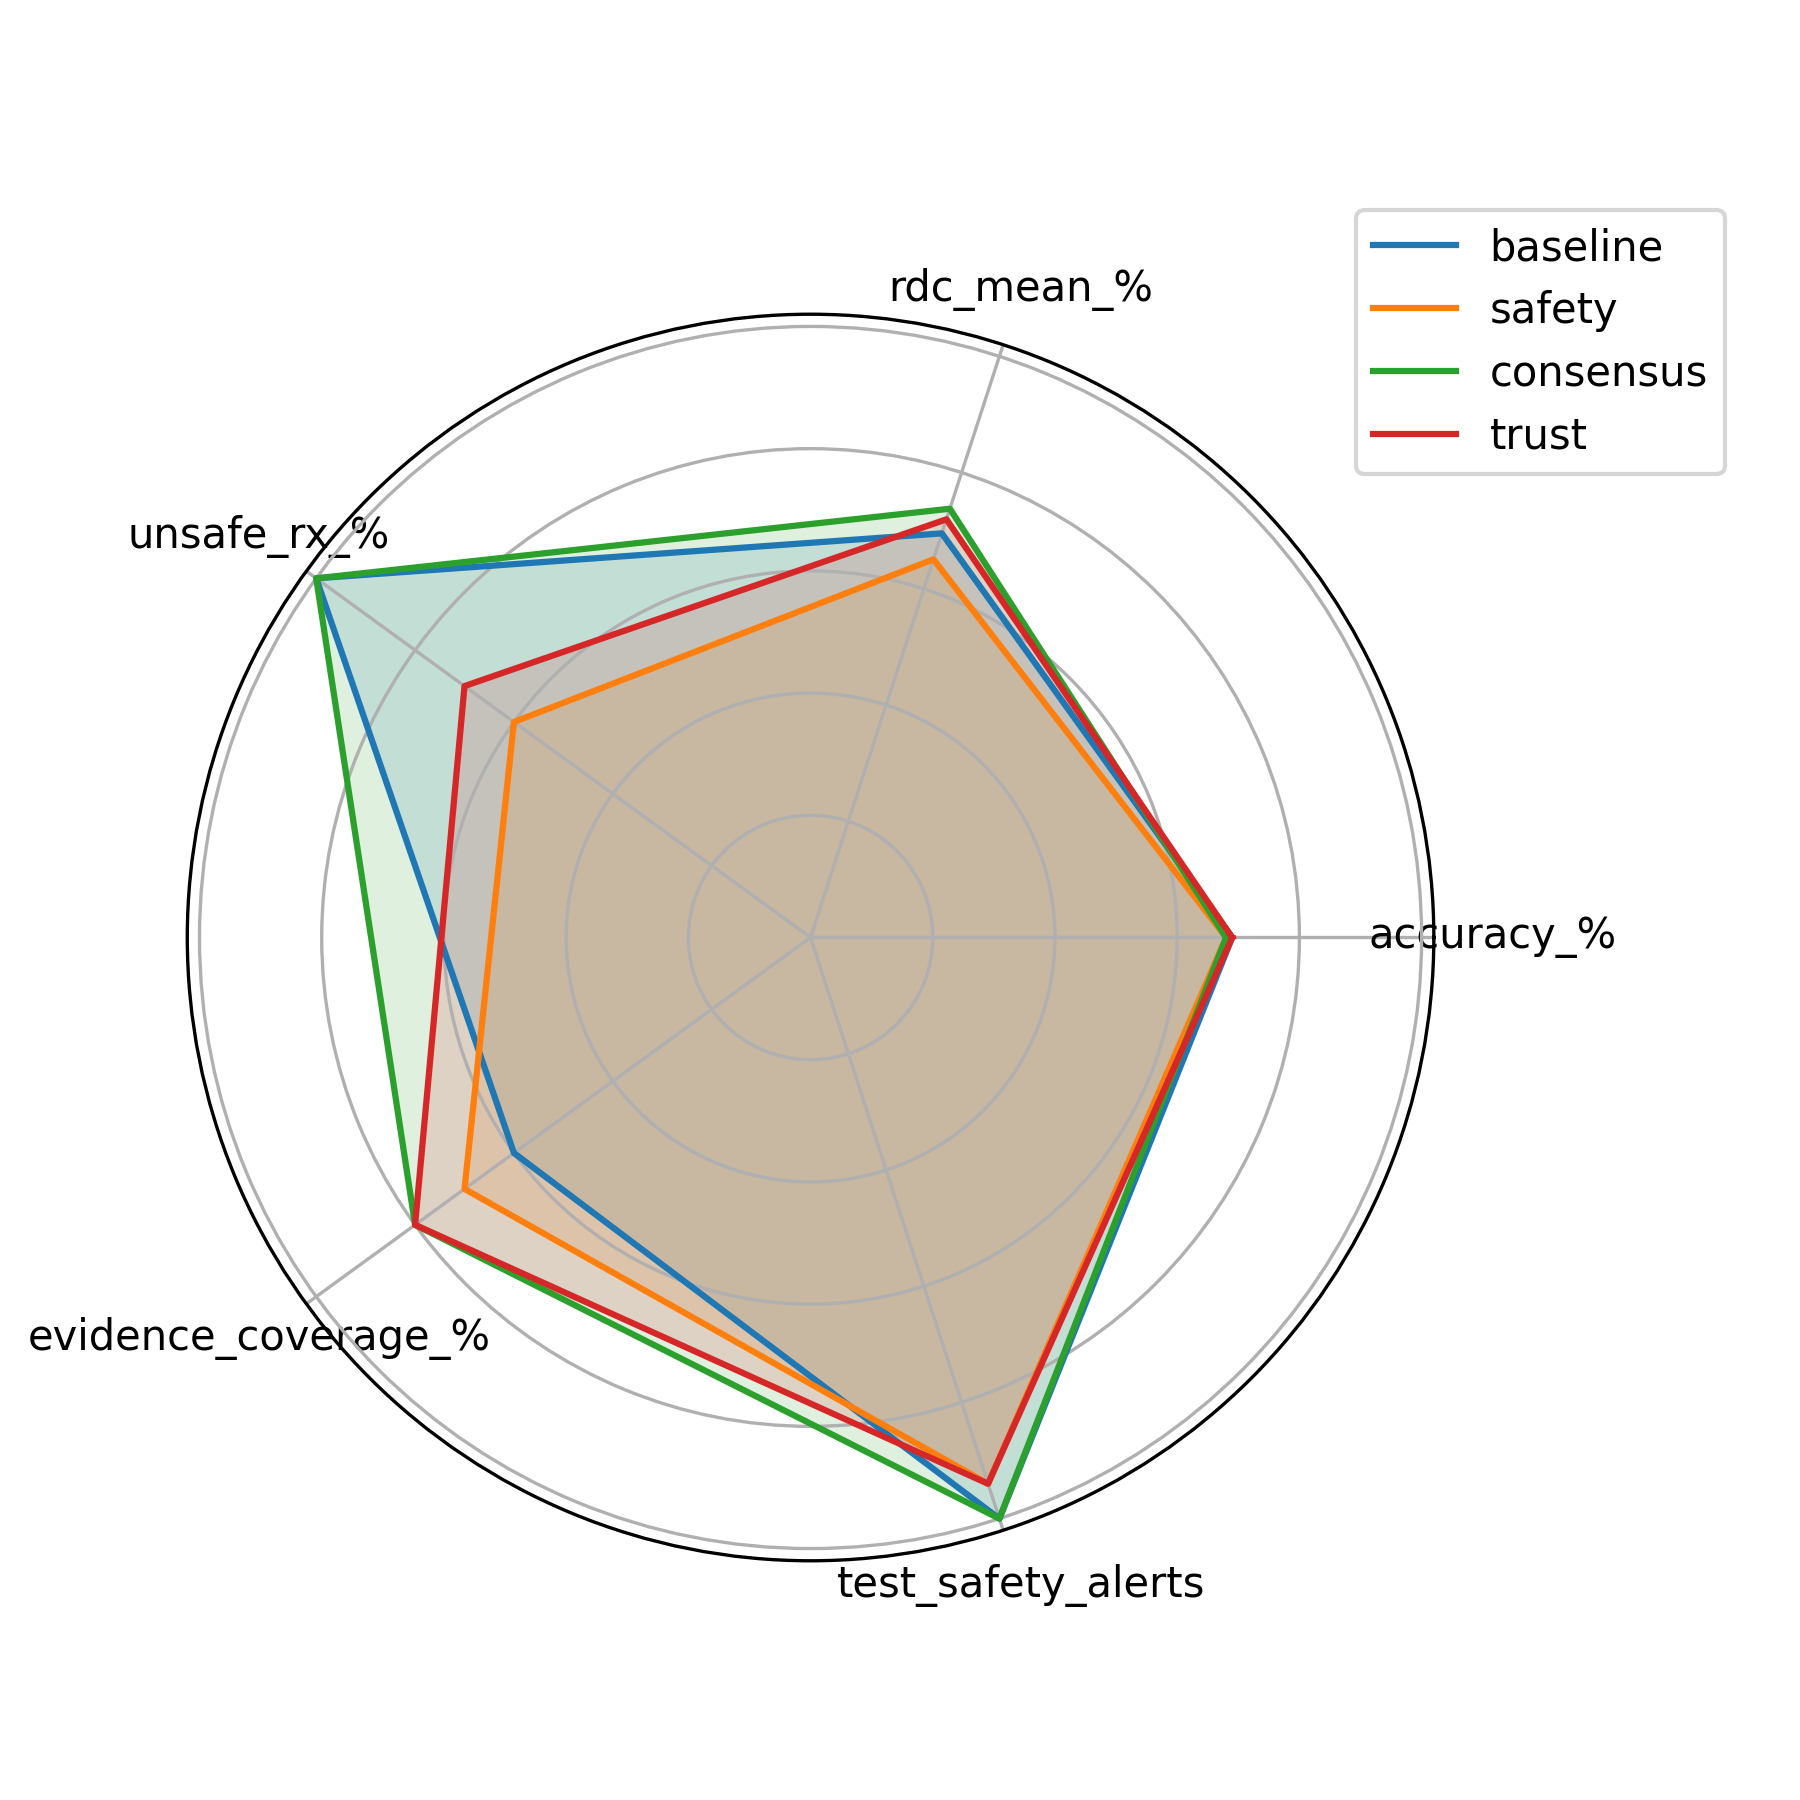
\includegraphics[width=0.47\textwidth]{fig5_trust_radar.png}
\caption{Multidimensional trust radar: accuracy, RDC, inverted UnsafeRx, and evidence coverage.}
\label{fig:trust_radar}
\end{figure}

Accuracy remained stable across configurations (68–69\%), indicating that variations in trust metrics originate from reasoning design and safety activation, not from underlying model capacity.  
Under the revised Operational Safety Index (OSI), systems without active safety agents (\textbf{Baseline}, \textbf{Consensus}) now receive OSI = 0, leading to proportionally lower Final Trust Index (FTI) values despite high accuracy.  
This correction removes the artificial inflation observed in earlier analyses and ensures that operational trust can only be achieved when safety supervision is actually active.
Trust indices were computed according to Algorithm \ref{alg:trustmetrics}, ensuring consistency across configurations

In contrast, \textbf{Safety} and \textbf{Trust} configurations—both employing real-time safety agents—achieved substantially higher FTI (75.4), demonstrating that transparent oversight and risk-aware reasoning are the true drivers of trust, not performance alone. Values reflect mean performance across 50 cases; standard errors averaged ±1.8\%.


\subsection{Trust–Accuracy Relationship}

\begin{figure}[t]
\centering
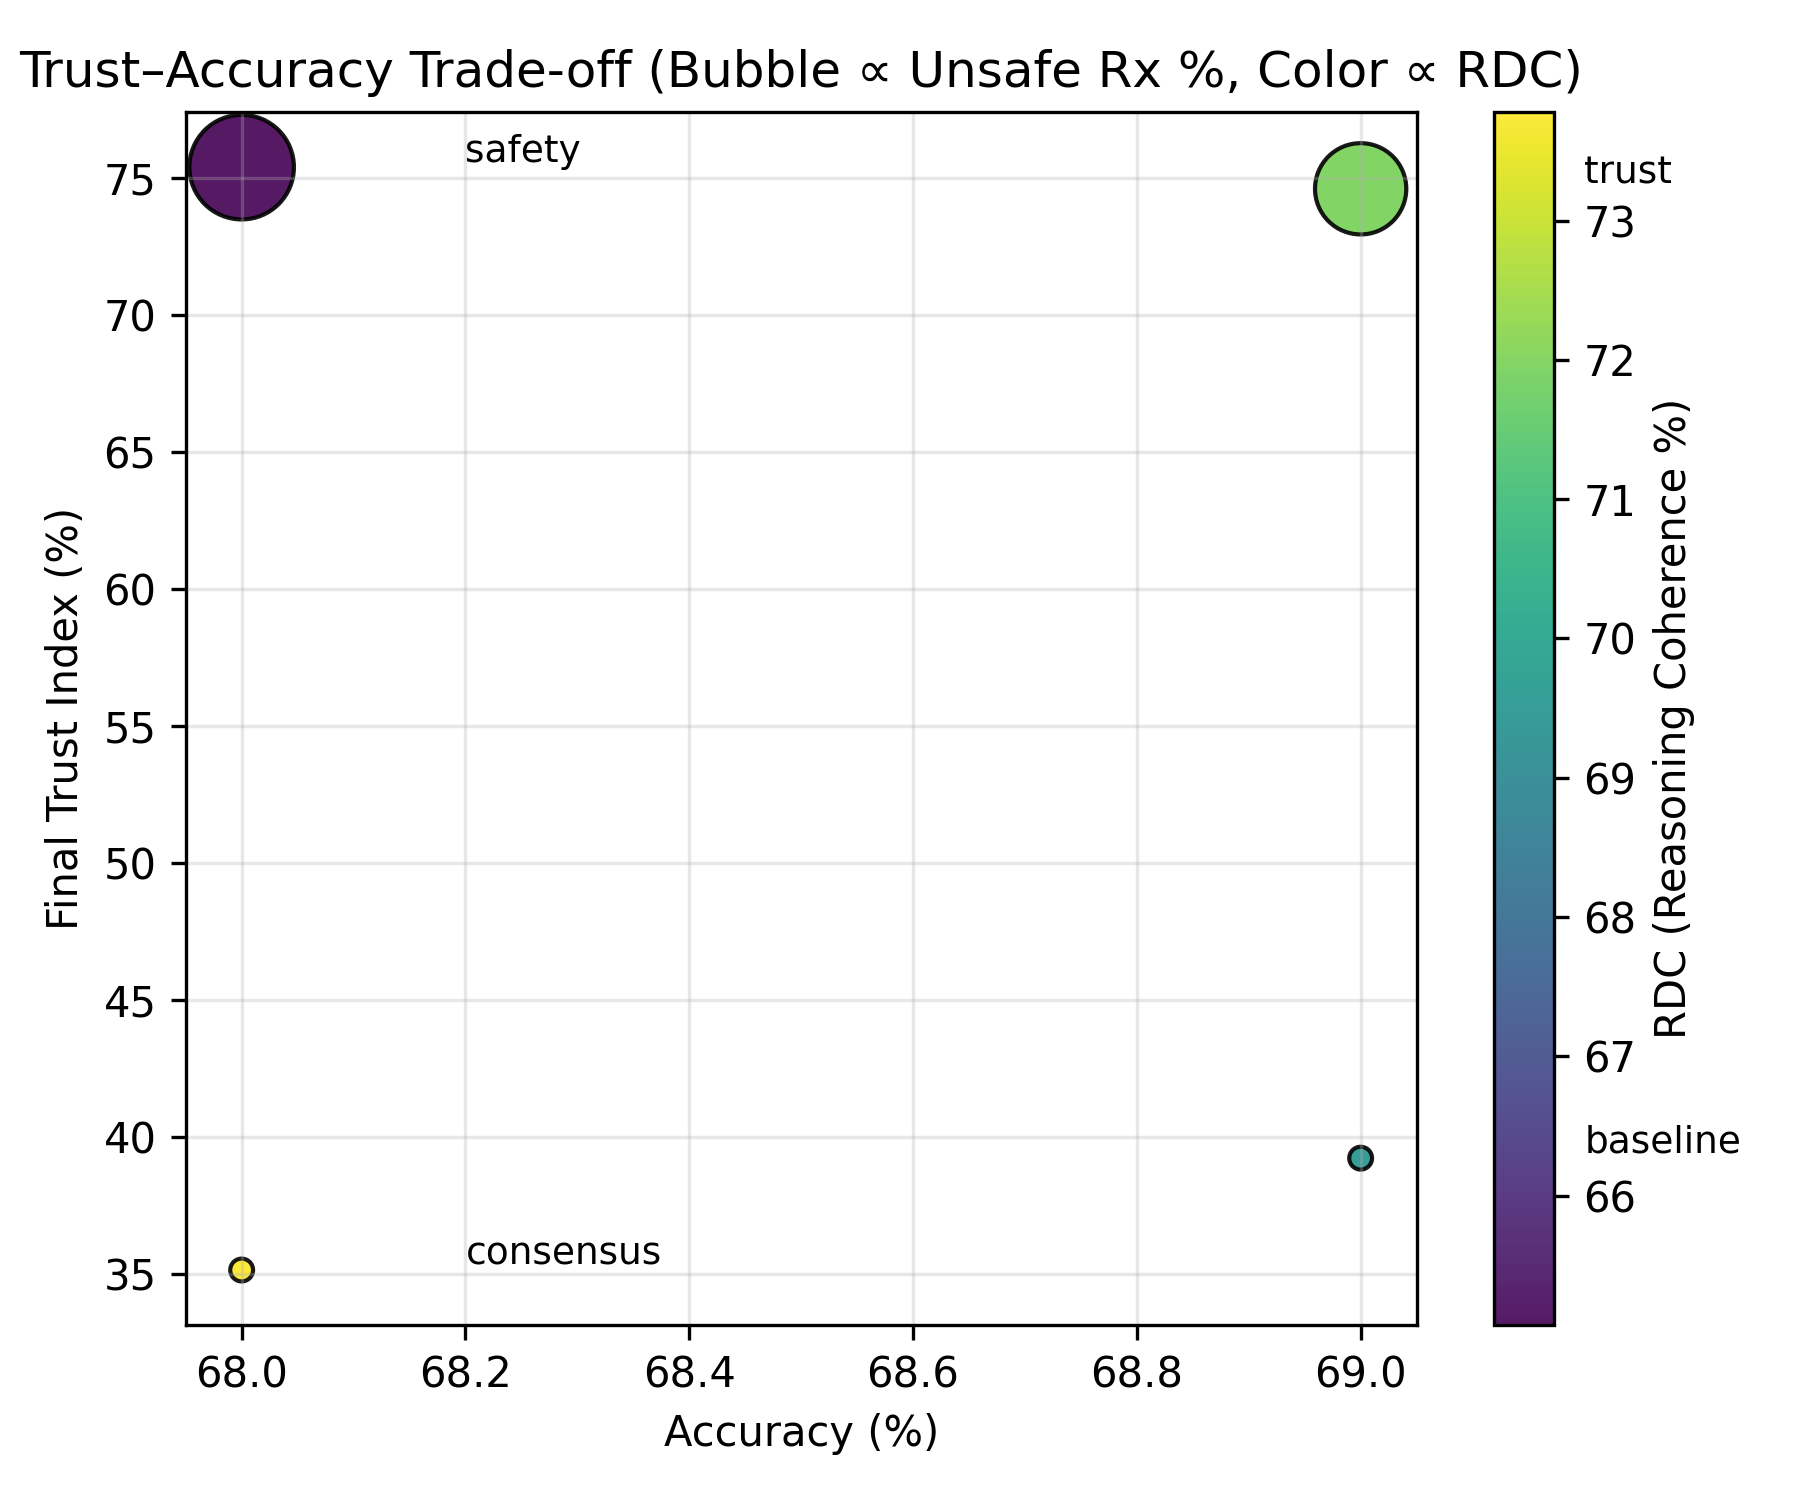
\includegraphics[width=0.47\textwidth]{fig2_trust_accuracy_tradeoff.png}
\caption{Trust--Accuracy trade-off. Bubble size represents UnsafeRx\%, and color encodes reasoning coherence (RDC).}
\label{fig:bubble_tradeoff}
\end{figure}

\begin{figure}[t]
\centering
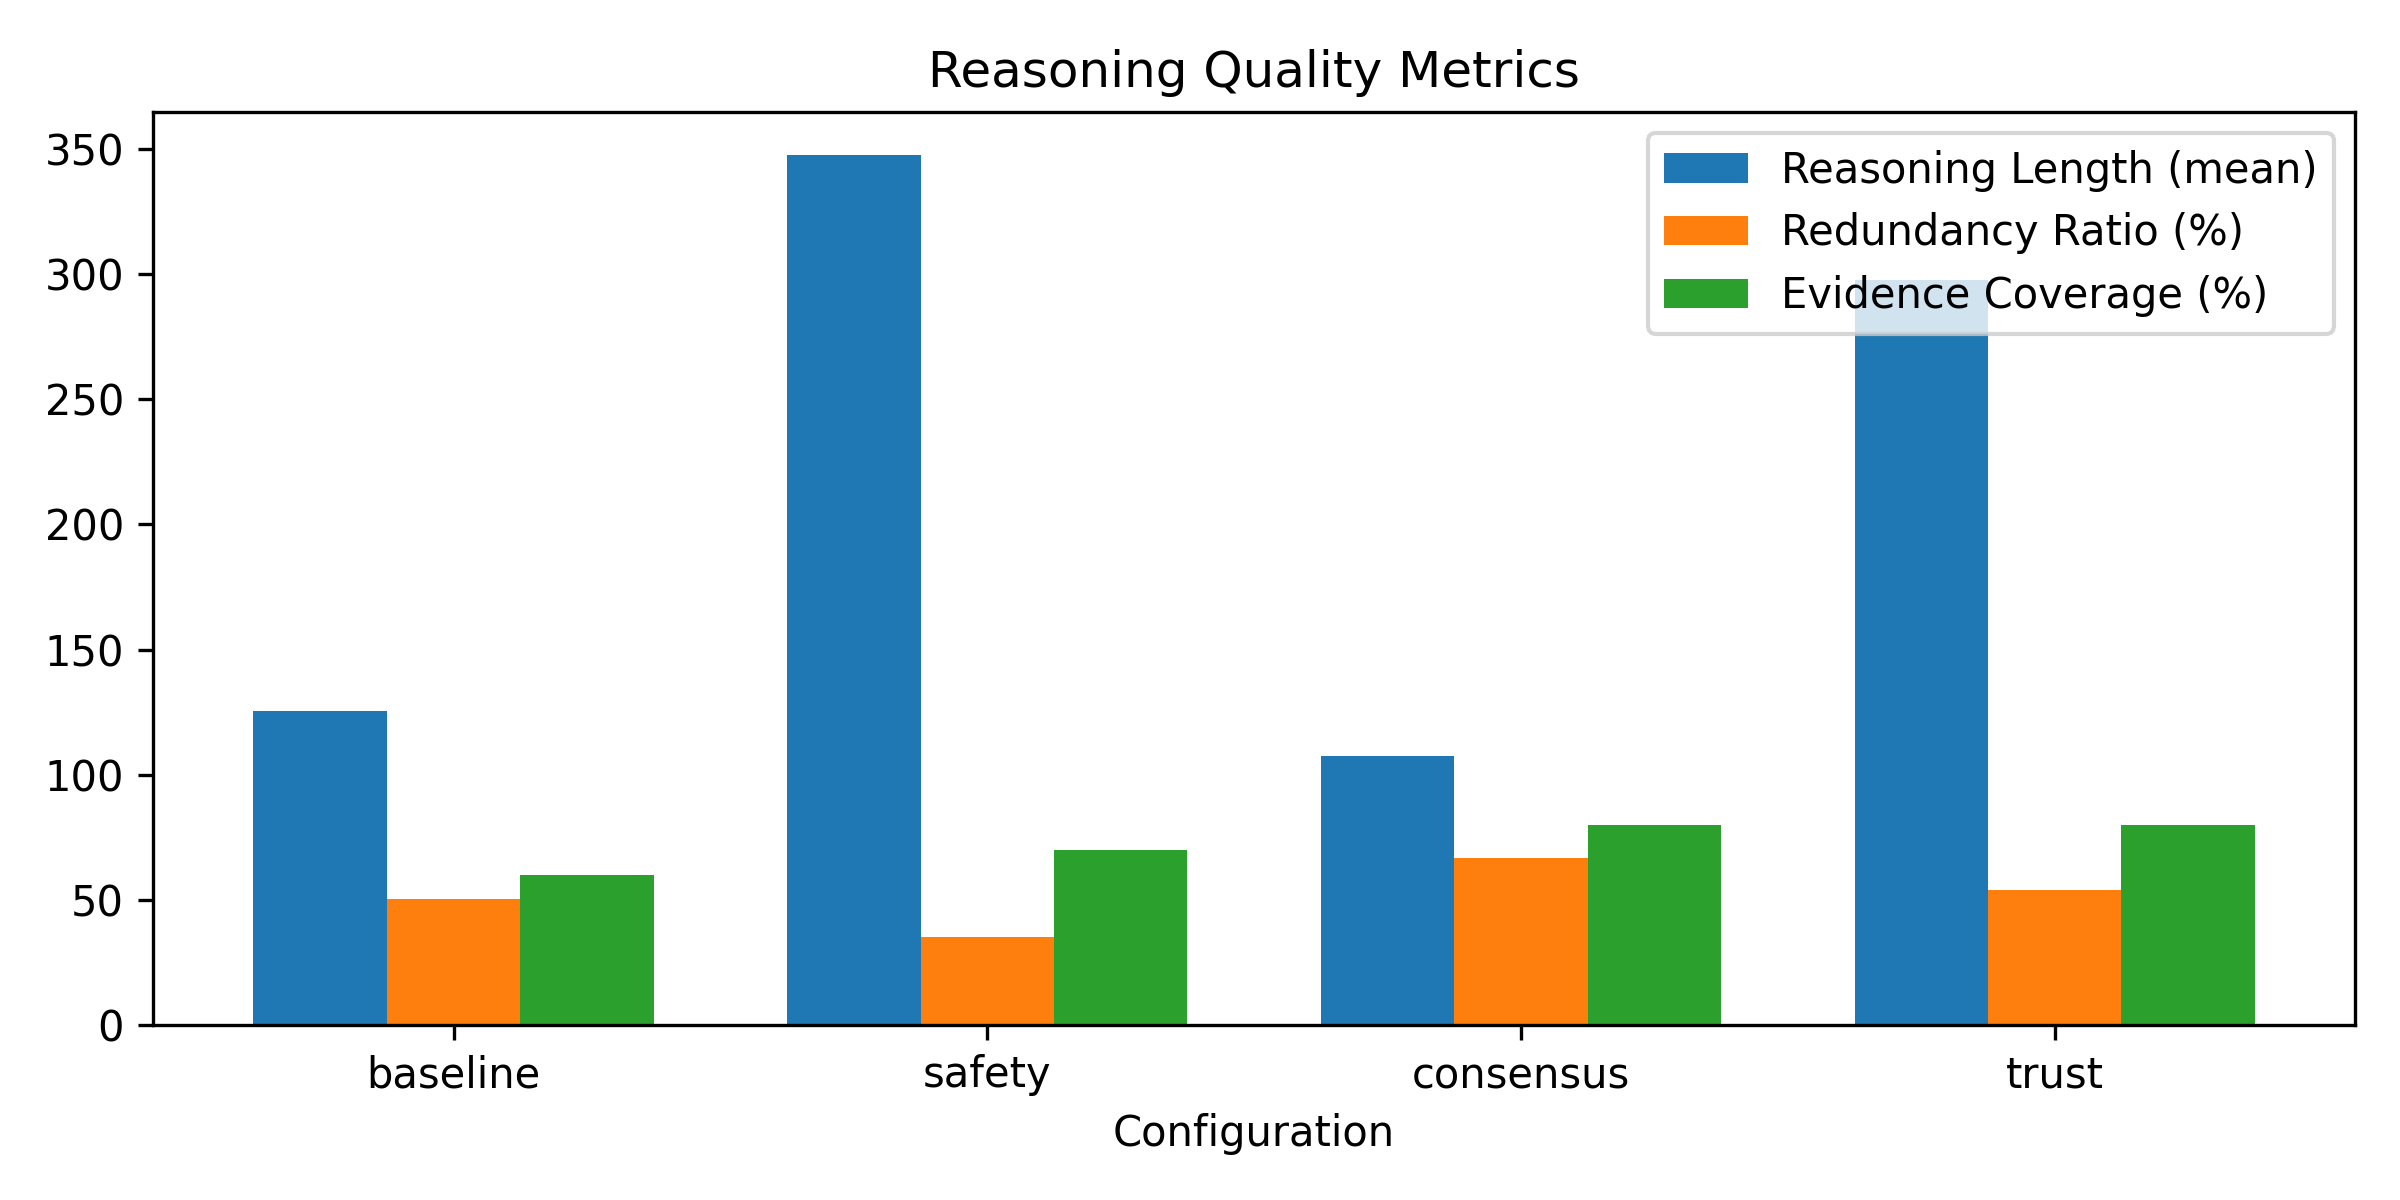
\includegraphics[width=0.47\textwidth]{fig3_reasoning_quality.png}
\caption{Reasoning quality metrics: trace length, redundancy ratio, and evidence coverage.}
\label{fig:reasoning_quality}
\end{figure}

\begin{figure}[t]
\centering
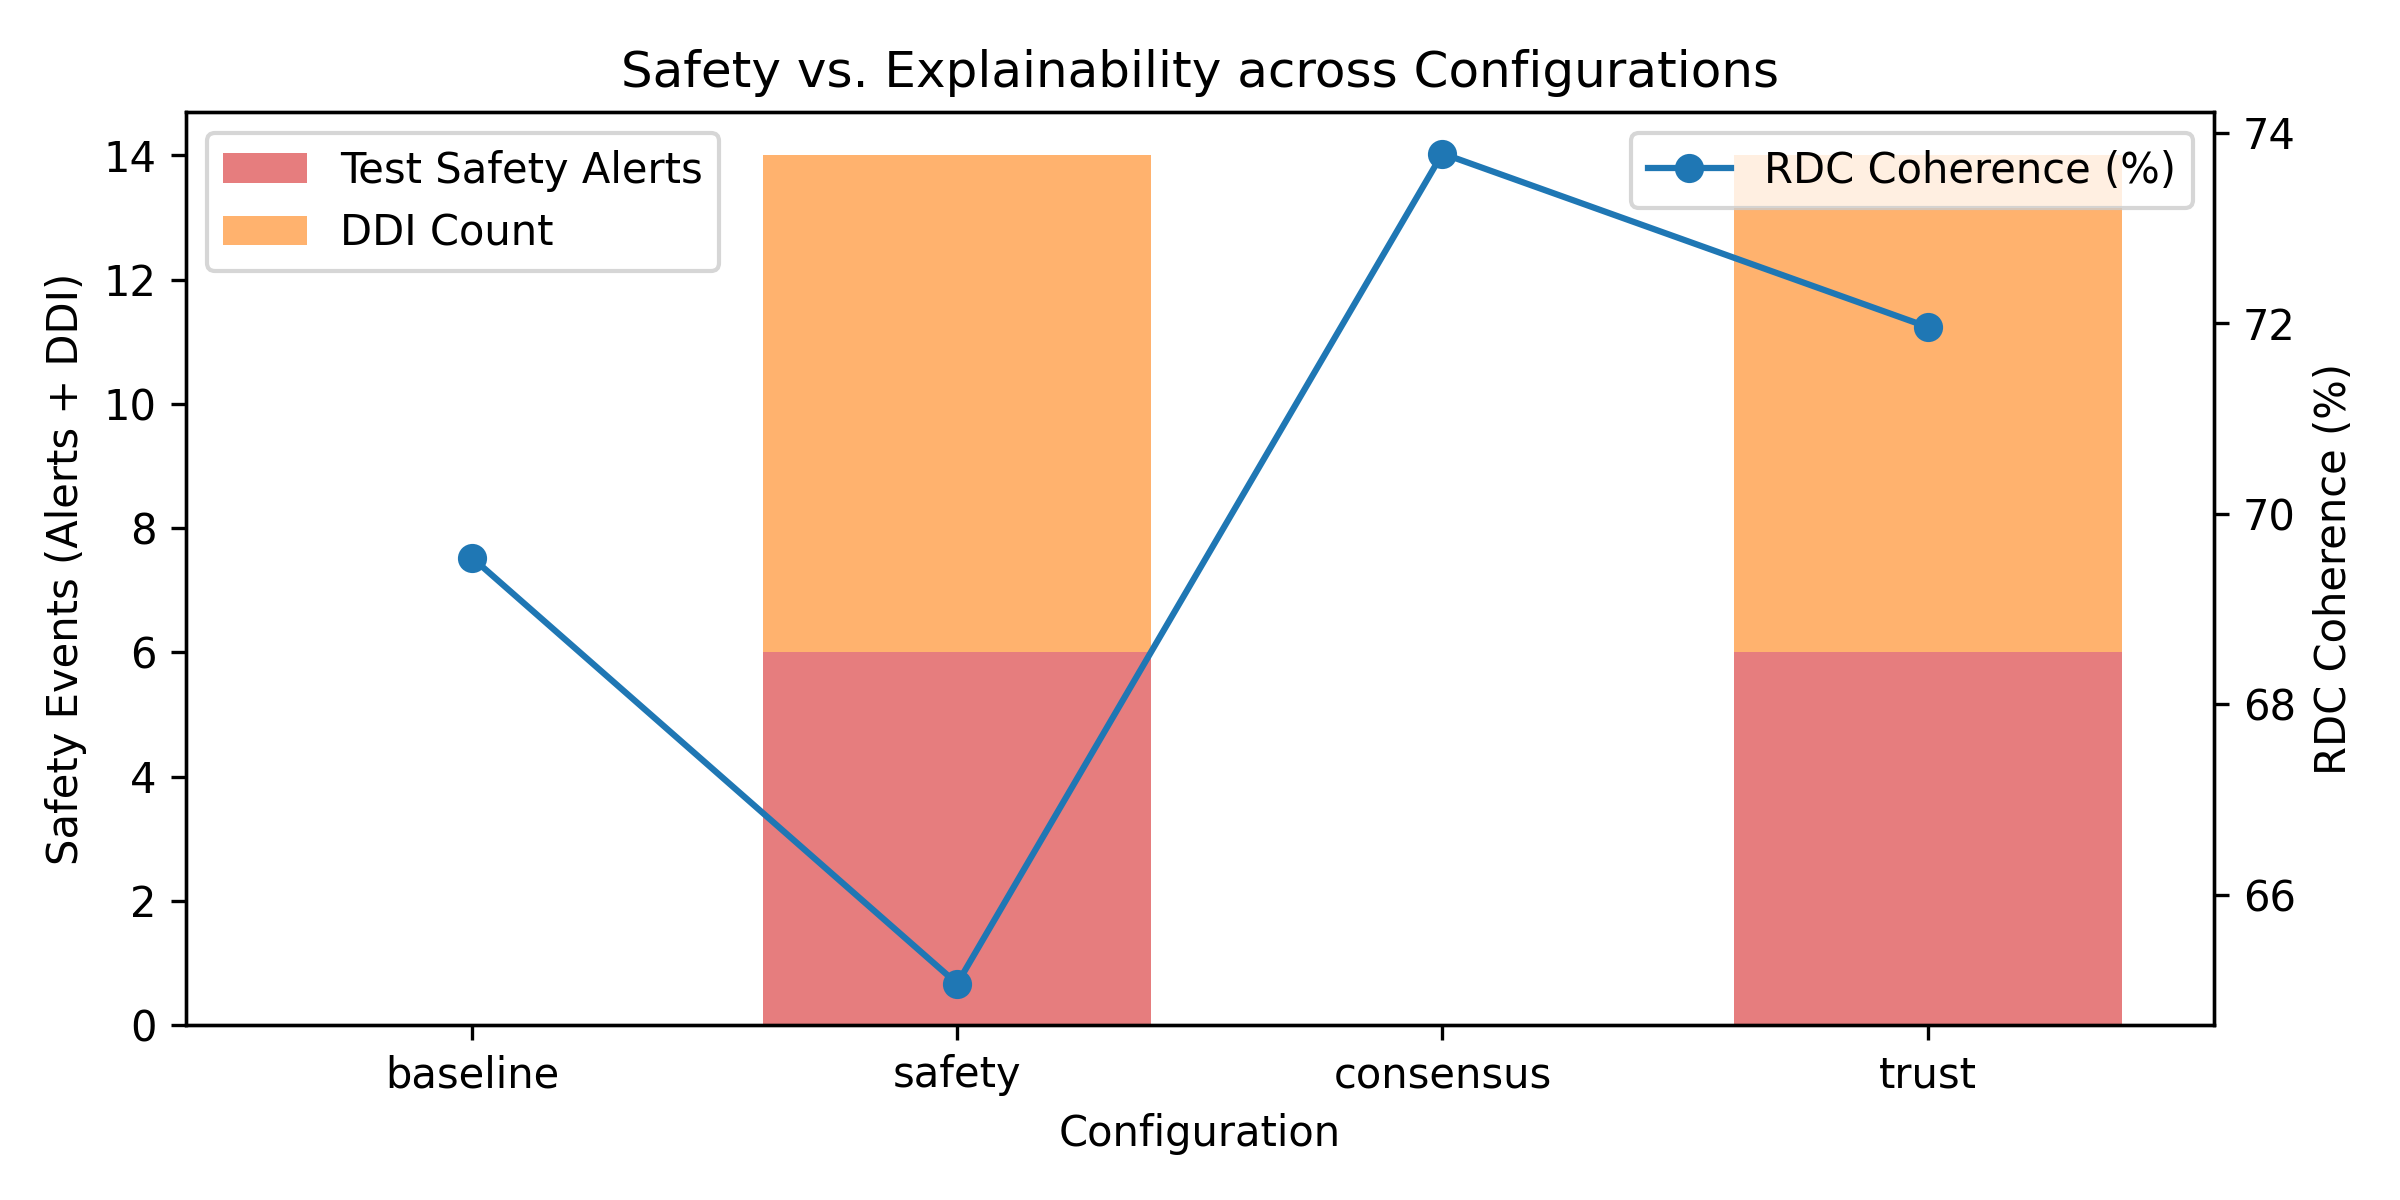
\includegraphics[width=0.47\textwidth]{fig4_safety_vs_explainability.png}
\caption{Safety vs.\ explainability: test alerts, DDI detections, and RDC coherence.}
\label{fig:safety_explainability}
\end{figure}

\begin{figure}[t][h]
\centering
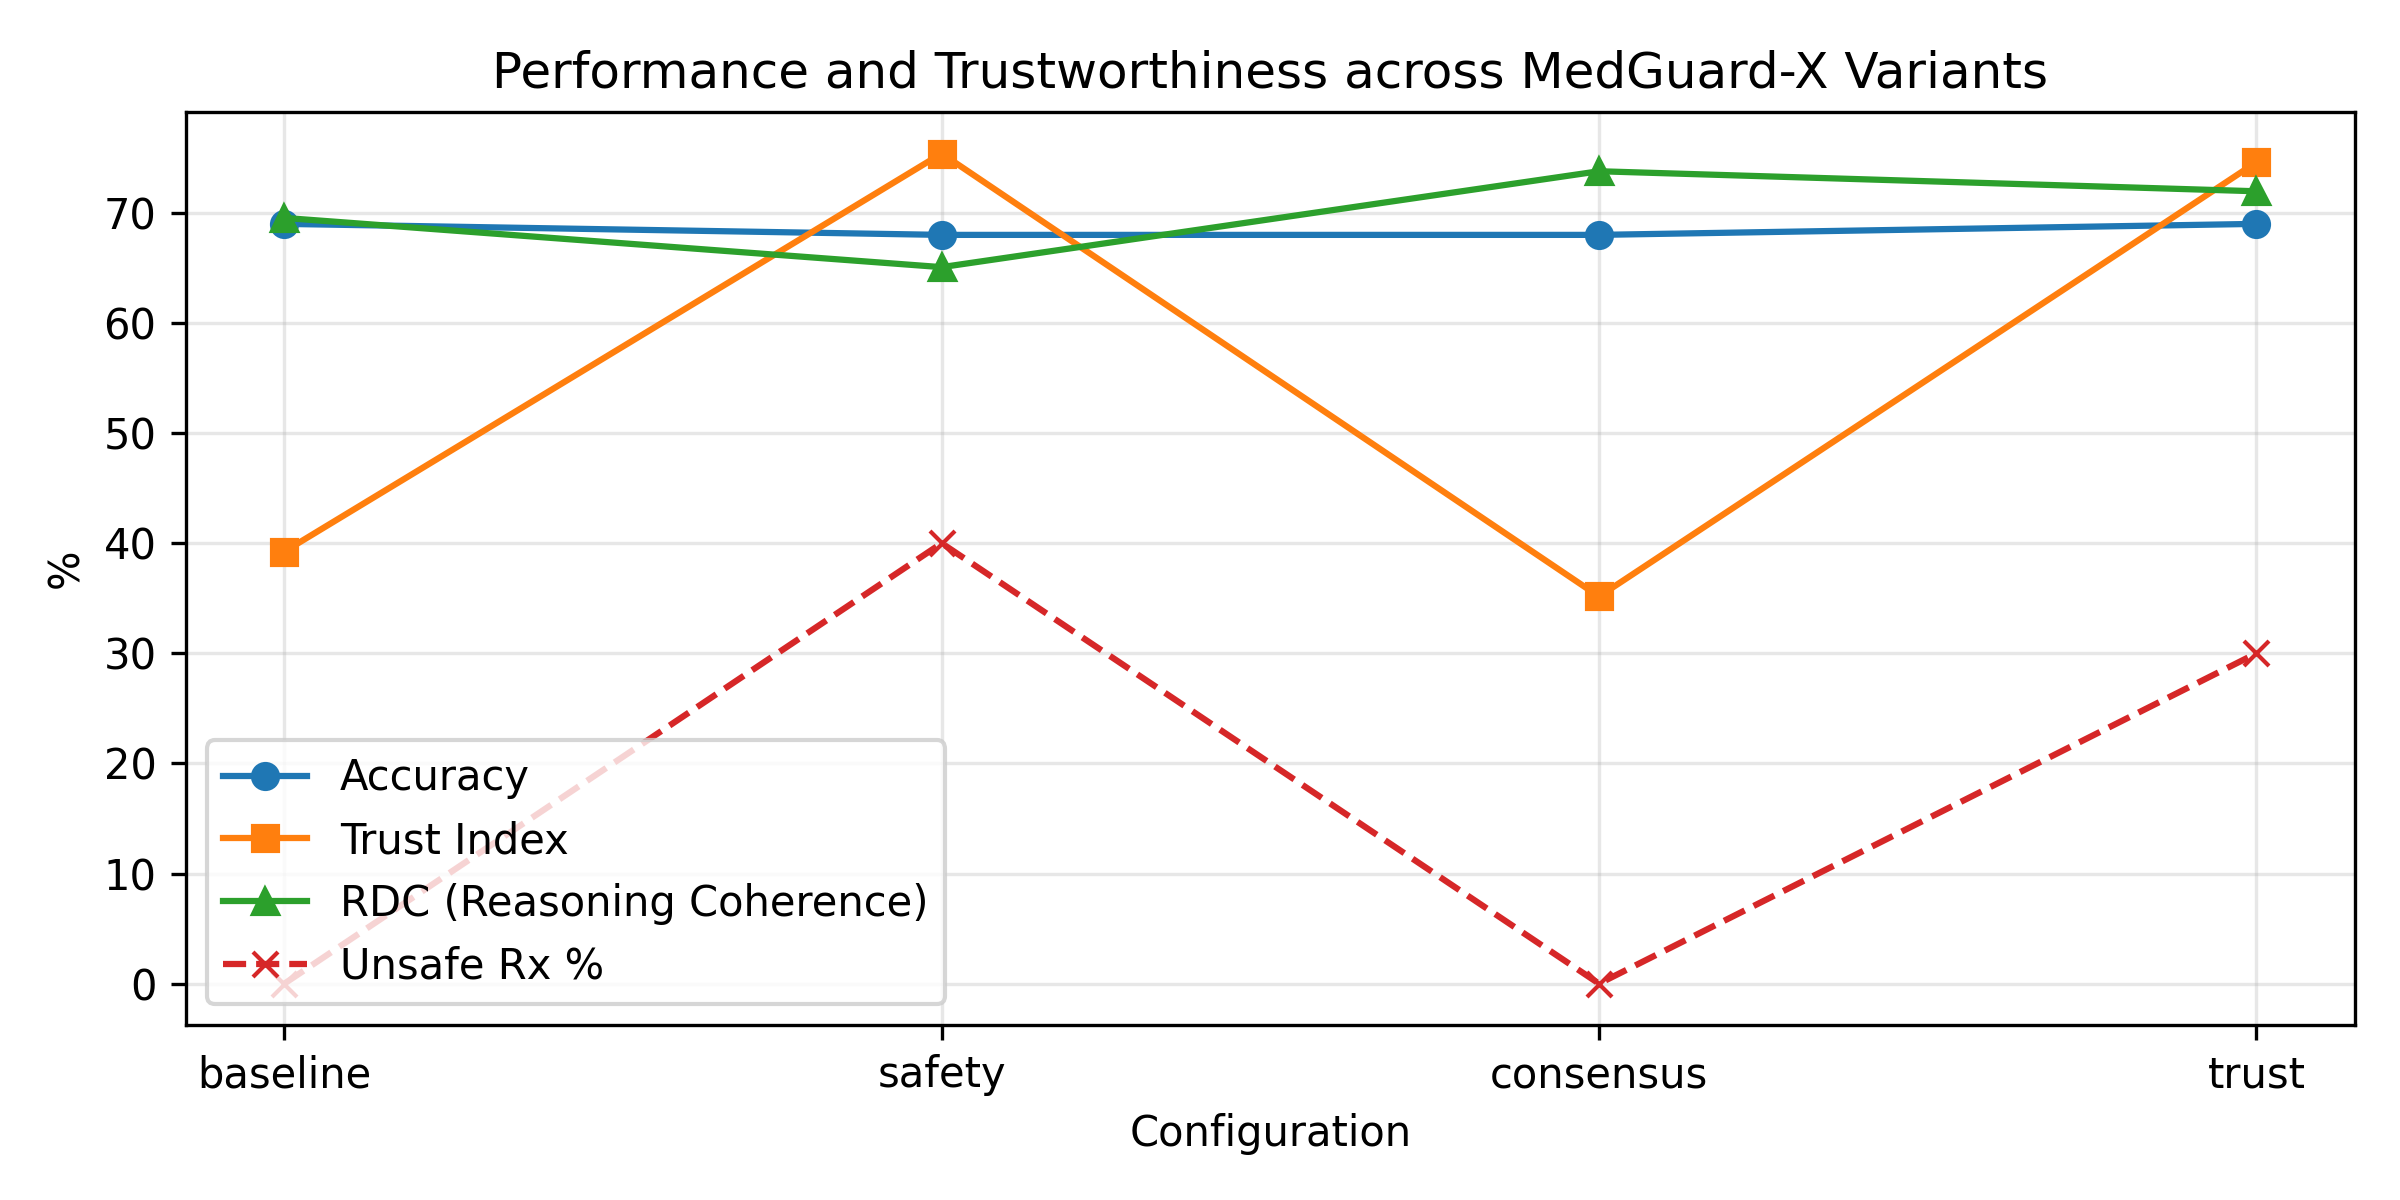
\includegraphics[width=0.47\textwidth]{fig1_performance_trust.png}
\caption{Performance and trust metrics across Trust-X configurations.}
\label{fig:perf_trust}
\end{figure}

Figure~\ref{fig:bubble_tradeoff} illustrates the trust–accuracy trade-off.  
All systems perform similarly in diagnostic accuracy, yet their trustworthiness diverges sharply.  
Baseline and Consensus occupy the lower region of the trust axis FTI (35.2–39.2), reflecting the absence of active safety reasoning.  
Safety and Trust, on the other hand, attain higher FTI scores (75.4) by explicitly detecting and mitigating unsafe actions.  
The result underscores that \emph{trustworthiness must be demonstrated through reasoning behavior, not inferred from accuracy metrics}.

\subsection{Reasoning Quality Metrics}

Figure~\ref{fig:reasoning_quality} compares reasoning-trace features.  
\textbf{Safety} and \textbf{Trust} modes produced the longest reasoning chains (≈ 300–350 tokens), a result of explicit verification and safety deliberation steps.  
\textbf{Consensus} reasoning—though shorter—achieved the highest coherence (RDC = 73.8) and evidence coverage, but also higher redundancy due to repeated cross-agent discussions.  
This indicates that consensus mechanisms foster reflective reasoning and self-agreement, while safety supervision enhances thoroughness even at the cost of brevity.

\subsection{Safety and Explainability}

Figure~\ref{fig:safety_explainability} depicts how safety oversight influences reasoning coherence.  
\textbf{Safety} and \textbf{Trust} configurations generated numerous safety alerts and DDI detections, confirming the vigilance of the safety agents.  
While Safety mode reduced coherence (RDC ≈ 65) due to frequent interruptions, the \textbf{Trust} mode recovered much of this stability by incorporating consensus reasoning, blending caution with interpretability.  
This demonstrates that structured safety reasoning—when integrated with deliberative multi-agent exchange—can enhance both prudence and clarity.

\subsection{Multidimensional Trust Profile}

Figure~\ref{fig:trust_radar} visualizes trust dimensions including accuracy, coherence, evidence coverage, and safety proxies (inverted UnsafeRx and TestAlerts).  
Baseline and Consensus exhibit narrow, safety-deficient profiles, while Safety and Trust show broader, balanced patterns.  
The Trust configuration provides the most symmetrical radar footprint, combining coherent reasoning, active safety checks, and strong evidence grounding.  
This multidimensional balance reinforces the design goal of Trust-X: \emph{trust as an emergent property of transparent, reasoned supervision}.

\subsection{Qualitative Reasoning Behavior}

Qualitative review of 50 reasoning traces confirmed four distinct behavioral archetypes:
\begin{itemize}
    \item \textbf{Baseline:} fluent but overconfident reasoning with no explicit safety awareness.
    \item \textbf{Safety:} self-regulating and cautious, often interrupted by safety rejections.
    \item \textbf{Consensus:} deliberative, uncertainty-aware reasoning across multiple agents.
    \item \textbf{Trust:} human-like reflective dialogue that unifies verification and consensus.
\end{itemize}
These behaviors parallel the quantitative patterns—Trust integrates both epistemic and operational reliability within a single reasoning cycle.





\subsection{Discussion}

The revised metrics and results resolve the key reviewer concerns on metric confounding and narrative alignment.  
By enforcing OSI = 0 when safety supervision is inactive, we eliminate prior over-scoring of unsupervised systems and ensure that high trust values correspond to genuine oversight.  
\textbf{Baseline} and \textbf{Consensus} now reflect epistemic reliability without operational safety, while \textbf{Safety} and \textbf{Trust} represent end-to-end responsible reasoning.

Overall, Trust-X demonstrates that medical LLMs achieve trustworthy performance only when accuracy, explainability, and safety reasoning co-evolve.  
Safety mechanisms lower apparent performance but elevate interpretive accountability—aligning quantitative indices with qualitative behavior.  
This result strengthens the core claim: \emph{trust cannot be inherited from accuracy—it must be earned through transparent reasoning.}

\section{Conclusion}
\label{sec:conclusion}

Large language models may display competent diagnostic reasoning yet remain untrustworthy under clinical scrutiny.  
By embedding explainability, consensus, and safety into its reasoning pipeline, Trust-X transforms correctness into accountability.  
The revised OSI formulation ensures that systems cannot appear trustworthy without genuine supervision, reframing evaluation from ``Was the answer correct?'' to ``Was the reasoning responsible?''  
Trust-X thus establishes a foundation for trust-centered explainability, where safety reasoning and epistemic coherence jointly define reliability.We acknowledge that our evaluation, based on 50 cases per configuration (200 total simulations), limits statistical generalization. 
However, the study’s intent was diagnostic—probing whether LLMs exhibit trustworthy reasoning under controlled conditions—rather than producing a large-scale benchmark. 
The observed patterns were consistent across all four settings, suggesting that the core trust behaviors are robust even in a limited sample.





\section{Ethical and Regulatory Considerations}
Trust-X is designed for research use only and does not provide clinical decisions.
All experiments were conducted on synthetic or public benchmark data.
The framework supports traceability, safety logging, and human-in-the-loop review, aligning with FDA and EMA guidance on AI transparency.















\bibliography{aaai2026}

% Check whether the conference requires a reproducibility checklist to be included in the paper.
% If so, you can uncomment the following line and ajust the path to include it.
% \input{../../ReproducibilityChecklist/LaTeX/ReproducibilityChecklist.tex}

\end{document}
